\chapter{Installation guide}
This installation guide guides you through how you install apps on the Arduino. If you are building your own Arduino, it is recommended to have programming expertise and know how serial communications works.\\

If you have bought a finished product, you can skip to the \ref{sec:install-android-application} section.

	\section{Upload the first application}
	Before you can use the $\mu$CSS, you need a standard application running on your Arduino, or else the Arduino will not be recognized as a supported device.
	
		\subsection{Arduino IDE}
		\begin{enumerate}
		\item To transfer the first application to your Arduino, you need the Arduino IDE. Download the latest version of Arduino IDE from \url{http://arduino.cc} and install this.
	
		\item Download the latest version of the ComputerSerial library from \url{https://github.com/Prosjekt2-09arduino/ArduinoStore/tree/master/Arduino/} and import this into Arduino IDE. How this is done, you can read here \url{http://arduino.cc/en/Guide/Libraries/}.
	
		\item Plug an USB cable into your Arduino and make sure you do not have anything plugged into the digital port 0 and 1, where the Bluetooth module usally is plugged into. This is because these pins are used for programming the device, and if you have something plugged in here the device will not get programmed over USB.
		\end{enumerate}
		
				
		\subsection{Configure Bluetooth module}
		To program the Arduino over Bluetooth the Arduino requires a baud rate at 115200. Standard configuration of Bluetooth modules is usally configured to use a lower baud rate, therefor it have to reprogramed it to use the correct baud.\\
		
		\begin{enumerate}
		\item Upload an application that does not use the serial communication. The Arduino IDE comes with a lot of example applications and you can use one of them, like Blink. This can be found in the menu (File -> Examples -> Basic -> Blink). Click the ''Upload'' button to upload.
		
		\item Switch the wires from the Bluetooth module (TX on the Arduino to TX on the Bluetooth module, same with RX), as shown in Figure~\ref{fig:arduino_configure_bluetooth}. This is done because the Bluetooth module have to communicate with the computer through the USB cable. Remember to switch the wires back when you are finished configuring, as shown in Figure~\ref{fig:arduino_standard_wiring}.
		
		\item Choose the right USB serial port from the menu.
		
		\item Open the serial monitor.
		
		\item Change from ''Newline'' to ''Both NL \& CR'' and change baud rate to the baud of the Bluetooth module, as shown in Figure~\ref{fig:serial_monitor}. If you are not sure what baud rate you should use, you can try different baud rates until you find the right.
		
		\item You are now ready to send commands to the Bluetooth module.
		\end{enumerate}
		
		\begin{figure}[H]
			\centering
			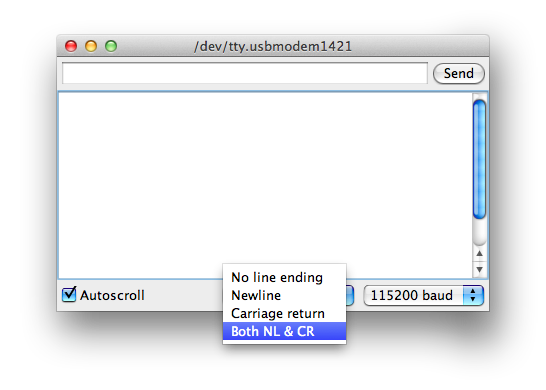
\includegraphics[scale=0.5]{images/serial_monitor.png}
			\label{fig:serial_monitor}
			\caption{Change settings in the serial monitor in the Arduino IDE to configure the Bluetooth module.}
		\end{figure}
		
		\begin{figure}[H]
		\subfigure[]{
			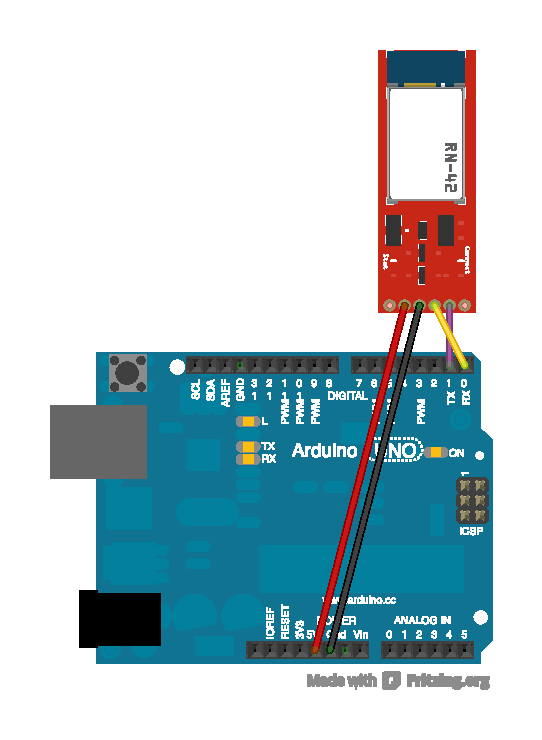
\includegraphics[width=0.5 \textwidth]{images/arduino_wiring.pdf}
			\label{fig:arduino_standard_wiring}
			}
		\hfill
		\subfigure[]{
			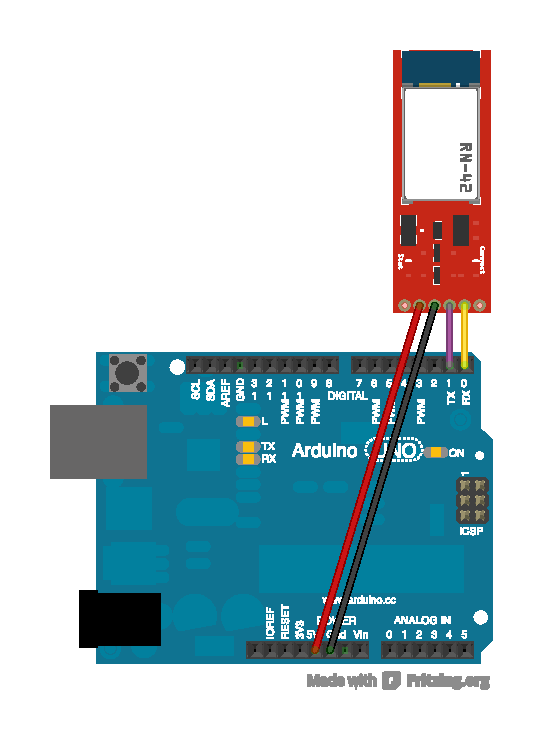
\includegraphics[width=0.5 \textwidth]{images/arduino_configure_bluetooth.pdf}
			\label{fig:arduino_configure_bluetooth}
			}
		\caption{Standard wiring of Bluetooth module: \protect{\ref{fig:arduino_standard_wiring}}. To configure the Bluetooth module through the Arduino, wire the module like this: \protect{\ref{fig:arduino_configure_bluetooth}}.}
		\end{figure}

			\subsection{Supported Bluetooth modules}
			You can use any Bluetooth module you want, but this is the modules that have been tested. Remember to power off the modules after they are reprogrammed to activate the new configuration.\\
			
			When the Bluetooth module is programmed, turn of the power and on again to restart the module. Load a test application from the ComputerSerial library. The examples can be found in the menu (File -> Examples -> ComputerSerial -> Examples).
			
				\subsubsection{RN-42}
				To enter programming mode, write ''\$\$\$'' and enter. You should get AOK back when you entered programming mode. To change baud to 115200, write SU,11 and hit enter. You should now get AOK back.\\
				
				Other supported commands can be found here \url{https://www.sparkfun.com/datasheets/Wireless/Bluetooth/rn-bluetooth-um.pdf}.

				\subsubsection{HC-05}
				Make sure you pull the KEY pin to 3.3v/5v (depends on what model of this module you have) before powering it up. This will allow you to enter the programming mode.\\
				
				After you have successfully connected to the Bluetooth module, just write ''AT'' and enter. You should get AOK back when you entered programming mode. To change baud to 115200, write ''AT+UART=115200,0,0''. You should now get AOK back.\\
				
				Other supported commands can be found here \url{http://elecfreaks.com/store/download/datasheet/Bluetooth/HC-0305%20serail%20module%20AT%20commamd%20set%20201104%20revised.pdf}.
				
	\section{Android application}\label{sec:install-android-application}
	To be able to install the Android application on your device, you have to allow installation of applications from unknown sources on the device. On Android 4.x, this option can be found in the security settings on the device. In the security menu, check the box next to ``Unknown sources''. \\

	To install the application on your device, you have to transfer the ``uCSoftwareStore.apk'' file to the device. This file can be found the provided CD. Once the file is transferred, press the file to install the application, and follow the on-screen instructions.
	
	\section{Develop your own apps}
	To learn more about how the Arduino works, take a look at the tutorials here \url{http://arduino.cc/en/Tutorial/HomePage}.\\
	
	To make your applications work with the $\mu$CSS, remember to always import the ComputerSerial library. Take a look at the included examples in the ComputerSerial library to understand how it works.